\begin{figure}[H]
	\centering
	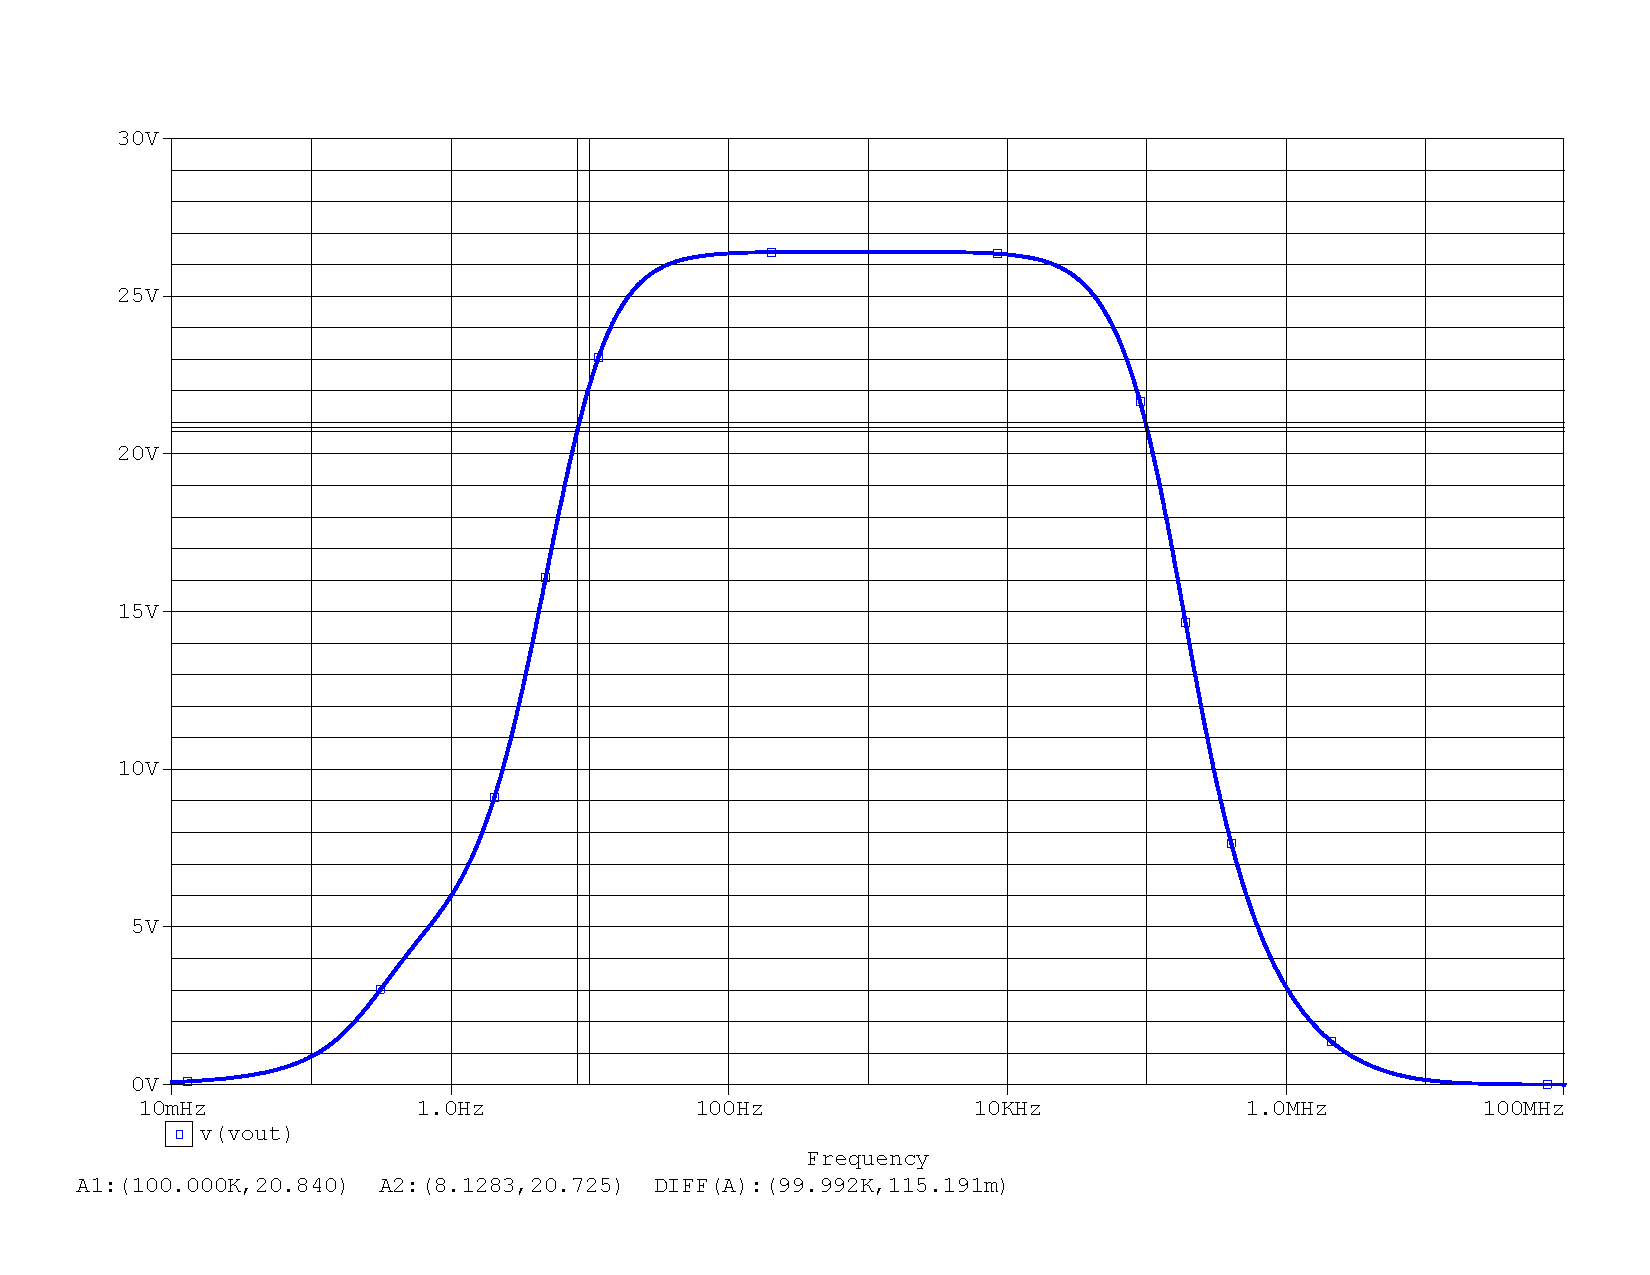
\includegraphics[scale=0.5]{sim_bw_potencia.pdf}
	\caption{Ancho de banda de potencia}
	\label{fig:sim_bw}
\end{figure}

El ancho de banda de potencia indica la máxima frecuencia para la cuál el amplificador logra reproducir una señal sinusoidal a máxima potencia. Para este caso, la máxima tensión sin distorsión apreciable es aproximadamente \SI{26}{\volt}. A partir de la figura \ref{fig:sim_bw} se obtiene

\begin{align}
	\centering
	f_L &= \SI{6.3}{\hertz} \\
	f_H &= \SI{120}{\hertz}
\end{align}
